\chapter{Education}
\label{chap:education}

\inspirationalquote{Knowing the students might one day
%find a way to
fix their concurrency bugs...
it fills you with determination.}{Undertale (paraphrased)}

Concurrency is taught in as many different ways as there are
systems programming classes at universities which teach the subject.
Yet one thing they all have in common is presenting the concurrency bug
as some elusive menace,
against which humanity's best weapon is mere random stress testing.
This chapter will prove stateless model checking's mettle as a better alternative in the educational theatre.

While the previous chapter demonstrated Landslide's bug-finding power
compared to prior MC techniques in a controlled environment,
whether it offers pedagogical merit in the hands of students and/or TAs is a separate question.
And while my MS thesis~\cite{landslide} showed that students
could annotate P3 Pebbles kernels and thence use Landslide to debug them,
the annotations alone required 2 hours of effort on average per user,
meaning the only students who could benefit were the ones already succeeding enough to have such free time.
% TODO: sect ref
Since then, I have extended Landslide with a fully-automatic instrumentation process
for Pebbles thread libraries (P2s) and Pintos kernels
to improve its accessibility.

I have run several user studies in the Operating Systems classes
at Carnegie Mellon University (CMU), University of Chicago (U. Chicago), and Penn State University (PSU),
wherein students get to use Landslide to find and diagnose their own bugs during the semester.
% TODO: put section refs
At CMU, I recorded logs and code snapshots as students used Landslide during P2.
At CMU and PSU, I surveyed students on their experience after submitting their Landslide-debugged P2s.
At U. Chicago, I collaborated with a TA to check submitted Pintos kernels,
then returned any resulting bug reports to students and likewise surveyed them on the quality of the diagnostic output.

%%%%%%%%%%%%%%%%%%%%%%%%%%%%%%%%%%%%%%%%%%%%%%%%%%%%%%%%%%%%%%%%%%%%%%%%%%%%%%%%

\section{Pebbles}

This section presents the user studies done in
%CMU's 15-410 and PSU's \psuos classes,
%in semesters Fall 2015 to Spring 2018 and in Spring 2018 alone, respectively,
%taught by David Eckhardt and Timothy Zhu, respectively.
CMU's 15-410 in semesters Fall 2015 to Spring 2018,
taught by David Eckhardt,
and in PSU's \psuos in Spring 2018,
taught by Timothy Zhu.
In both cases the instructors assisted to introduce me during the guest lecture
%(see below)
and to distribute the recruiting emails;
TAs were not involved.
The in-house user study has CMU IRB approval under study number STUDY2016\_00000425,
and the external user study under STUDY2017\_00000429.

% Possible experiment questions
% compare e.g. use after free bug reporce from OOPSLA data set, to P2 grade files, see who has thread exit uafs
% is landslide better at finding thread uafs than TAs
% same Q for other stuff.. (expect paraguay answer to be "no", explain why)

\subsection{Recruiting}
\label{sec:education-pebbles-recruiting}

Since the Spring 2015 semester I have given a guest lecture in 15-410
to recruit students to participate in the user study.
The 50-minute lecture is given 1 week into the 2.5-week-long P2 project,
approximately when the students should be getting child threads running in {\tt thr\_create()}
and experiencing concurrency bugs for the first time.
It introduces the research subject abstractly
using an example ``Paradise Lost'' bug from a previous lecture \cite{paradise-lost},
explains how Landslide works concretely,
shows a short demo of effortlessly using Landslide to find the example bug,
and provides the necessary IRB legalese about the risks and benefits of participation.
The most recent lecture slides are available on the course website at
\url{http://www.cs.cmu.edu/~410-s18/lectures/L14_Landslide.pdf},
and all semesters' editions at
\url{https://github.com/bblum/talks/tree/master/landslide-lecture}.

The PSU version of the lecture
%was given in Spring 2018, and
is available at
\url{http://www.contrib.andrew.cmu.edu/~bblum/psu-lecture.pdf}
as well as under the github link above.
Being a 70-minute lecture slot rather than 50, I extended the demo to
both find and (attempt to) verify a fix for two bugs:
one a simple data race and the other the more complicated Paradise Lost bug as above.
After finding each bug, I demonstrated using Landslide on a fixed version of the code
to show how it proves the test case correct by completing all state spaces,
or (in the case of Paradise Lost) suffers an exponentially-exploding state space.
Not that I scientifically measured it or anything,
but this extended demo seemed to help students more clearly understand Landslide's intended workflow,
at the cost of about 10-15 extra minutes of lecture time.

At both schools students then signed up using a Google form I emailed them,
which upon completion linked them to the Landslide user guide,
which is available at
\url{http://www.contrib.andrew.cmu.edu/~bblum/landslide-guide-p2.pdf}
(CMU version)
and
\url{http://www.contrib.andrew.cmu.edu/~bblum/landslide-guide-psu.pdf}
(PSU version)
and
\url{https://github.com/bblum/talks/tree/master/irb}
(both versions).

\subsection{Automatic instrumentation}
\label{sec:education-pebbles-instrumentation}

As described in \sect{\ref{sec:landslide-setup}},
all setup from the user's point of view is handled through the {\tt p2-setup.sh} script%
\footnote{PSU's version is called {\tt psu-setup.sh};
in this section, unless otherwise noted, {\tt p2-setup.sh} will refer to both.
}.
It, its helper scripts (\sect{\ref{sec:landslide-glue}}),
and the {\tt landslide} script itself contain several checks to prevent
studence
from accidentally misusing Landslide in ways that could produce mysterious crashes, false bug reports, and so on
(the need for each one, as the reader might imagine, discovered through bitter experience).
These include:
\begin{itemize}
	\item {\tt p2-setup.sh} checks if the directory argument correctly points at the top-level P2 basecode directory
		rather than any subdirectories such as {\tt user/libthread/}.
	\item {\tt check-need-p2-setup-again.sh} checks if any source files in the original P2 source directory
		(the argument supplied to {\tt p2-setup.sh}),
		in case the student hoped to fix some bug and verify their fix but forgot to re-run the setup script.
	\item {\tt landslide} checks the supplied test name matches one of the endorsed Landslide-friendly tests
		(students love trying to run Landslide with {\tt racer}, {\tt largetest},
		or even the string {\tt OPTIONS}).
	\item {\tt landslide} checks if any other instance of itself is simultaneously running in the same directory,
		and if so, refuses to do so and advises the student
		to {\tt git clone} the repository afresh for simultaneous use%
		\footnote{This is ironically implemented with a non-atomic lock file
		and should really be using {\tt flock} instead.
		}.
\end{itemize}
\vspace{1em}

\noindent Landslide also includes several P2-specific instrumentations and features to cope with various student irregularities:
\begin{itemize}
	\item Quicksand emits different combinations of {\tt within\_function}/{\tt without\_function} directives
		for Landslide depending on the name of the test.
		For example, for {\tt paradise\_lost} Landslide will not preempt in a function named {\tt critical\_section()},
		which the test case uses to protect an internal counter used to detect the bug;
		and it will not preempt in any of the {\tt thr\_*()} thread library API functions
		for tests intended to target just the concurrency primitives.
		In future work this could be improved as annotations to be placed inside the test case code itself.
	\item Landslide finds ad-hoc synchronization patterns which students often open-code,
		rather than using the prescribed synchronization API,
		such as {\tt while (!flag) yield();} or {\tt while (xchg(...)) continue;},
		and treats them as synchronization points as described in \sect{\ref{sec:landslide-blocking}}.
	\item Landslide finds ``too suspicious'' spinwait-loops in the students' mutex implementations
		which are neither yield- nor {\tt xchg}-loops (as described above),
		which would ordinarily be classified as infinite loop bugs,
		and reports them with a suggestive message ({\tt undesirable\_loop\_html()} in {\tt landslide.c})
		referring them to the appropriate lecture material
		\cite{synchronization-2}.
	\item The {\tt landslide} wrapper script logs the time and command-line options of invocation
		and captures a snapshot of the student code and results of the test and saves them to AFS after each run.
		% HURDLE_VIOLATION -- no, this is for p3 (context switcher) features only
\end{itemize}

\subsection{Test cases}
\label{sec:education-pebbles-tests}

Landslide ships with several ``approved'' test cases,
i.e., programs copied from, derived from, or at least vaguely resembling
the tests distributed with P2,
which I curated to produce concurrent behaviour suitable for stateless model checking.
Some tests are crafted to target specific bugs which,
from personal experience as a TA, are common in many student submissions;
others are crafted to exercise generally concurrency-heavy code paths and uncover any number of unforeseen problems.
Many use some of the features/annotations described in \sect{\ref{sec:landslide-testcases}}.

\subsubsection{Test case list}

The following tests were released to CMU students:
\begin{itemize}
	\item {\tt broadcast\_test}:
		Tests the {\tt cond\_broadcast()} signalling path with a single waiter.
	\item {\tt mutex\_test}:
		Tests student mutexes under 2 threads with 2 iterations
		(the 2nd iteration serves to expose problems with {\tt mutex\_unlock()} as well as {\tt mutex\_lock()}).
		This test uses the {\tt TESTING\_MUTEXES}
		described in \sect{\ref{sec:landslide-staticconfig}}
		to enable data-race preemption points within the mutex implementation.
	\item {\tt paradise\_lost}:
		Written for the sake of the Landslide lecture demo
		(\sect{\ref{sec:education-pebbles-recruiting}}).
		Tests for the Paradise Lost bug by attempting to break mutual exclusion.
	\item {\tt paraguay}:
		Copied directly from the P2 test suite;
		tests for proper handling of seemingly ``spurious'' wakeups in {\tt cond\_wait()}.
		Written by Michael Sullivan.
	\item {\tt rwlock\_downgrade\_read\_test}:
		Copied directly from the P2 test suite;
		tests for mutually-exclusive and deadlock-free {\tt rwlock\_downgrade()}.
		Written by me (as a TA).
	\item {\tt thr\_exit\_join}:
		Copied directly from the P2 test suite;
		tests for a variety of problems between {\tt thr\_exit()} and {\tt thr\_join()},
		but especially for memory issues pertaining to stack deallocation.
\end{itemize}
\vspace{1em}

\noindent The following tests were released to PSU students, in addition to the ones above:
\begin{itemize}
	\item {\tt atomic\_compare\_swap}:
		Tests the {\tt cmpxchg} assembly function for being properly atomic.
		Uses the {\tt magic\_*} global variables described below, and invokes {\tt vanish()} directly,
		to avoid requiring the student to implement {\tt thr\_join()}/{\tt thr\_exit()}
		before being able to run this test.
	\item {\tt atomic\_exchange}:
		As above for {\tt xchg}.
	\item {\tt atomic\_fetch\_add}:
		As above for {\tt xadd}.
	\item {\tt atomic\_fetch\_sub}:
		As above for {\tt xadd}.
	\item {\tt broadcast\_two\_waiters}:
		As {\tt broadcast\_test}, but uses two waiting threads to ensure both get signalled.
\end{itemize}
\vspace{1em}

\noindent The tests can all be viewed at \url{https://github.com/bblum/landslide/tree/master/pebsim/p2-basecode/410user/progs}.

\subsection{Survey}
\label{sec:education-survey-pebbles}

Starting in Fall 2017, I sought to gauge the students' personal opinions on their experience with Landslide,
in addition to simply counting
from the automatic snapshots
how many bugs were found.
Shortly after the P2 submission deadline,
I asked participants to answer several survey questions, reproduced below.
%distributed via email as a Google Doc.

\begin{enumerate}
	\item How many bugs did Landslide help you find in your code? (Please indicate a number.)
	\item How many of the bugs you found with Landslide do you believe you fixed before submitting your project? (You may answer ``all'', ``none'', or a number.)
	\item How many of the bugs you found with Landslide did you verify you had fixed by running Landslide again to make sure the bug was gone? (You may answer ``all'', ``none'', or a number.)
	\item In addition to the bugs Landslide found, did it report anything that you believe was NOT a bug? For example, Landslide printed an execution trace that was actually impossible, or Landlside reported a bug about some behaviour that was actually allowed by the P2 specification. (If so, please describe.)
	\item I found Landslide's debugging output easy to understand.
		(Multiple choice from strongly disagree to strongly agree.)
	\item It's easier to diagnose the root cause of a bug with Landslide than with a stress test (e.g. juggle).
		(Multiple choice from strongly disagree to strongly agree; plus ``Not sure'' and ``Easier for some bugs but harder for others'')
	\item I felt the time I saved by having Landslide to help debug was worth the time it took me to learn how to use Landslide.
		(Multiple choice from strongly disagree to strongly agree.)
	\item I feel that by using Landslide I learned to understand concurrency better.
		(Multiple choice from strongly disagree to strongly agree.)
	\item Suppose after you submitted your project, % "P2" for cmu, "project" for pintos
		we gave you 100 CPU-hours on the cloud provider of your choice to test it. Then we extended the project deadline by a day for you to use the results to fix bugs and get partial credit. How would you divide that CPU time between the staff-provided stress tests and Landslide?
		(Multiple choice: 0/10/.../100 CPU-hours on Landslide, 100/90/.../0 CPU-hours on stress tests.)
	\item If I found out next semester that a friend of mine (or a student in my degree program) were taking OS, I would recommend that they should probably invest some time during the project % "P2" for cmu, as above
		to learn Landslide and try to find bugs with it.
		(Multiple choice from strongly disagree to strongly agree.)
	\item Regarding the previous question, why or why not?
\suspend{enumerate}
\vspace{1em}

\noindent The following questions were served only on the CMU version of the survey.
\resume{enumerate}
	\item Did you answer this survey together with your partner, or on your own while they were busy? (If you both have time for it, please try to submit one survey together.)
		(Multiple choice: together or alone)
	\item Your andrew ID
	\item Your partner's andrew ID (if any)
\suspend{enumerate}
\vspace{1em}

\noindent The following questions were served only on the PSU version of the survey.
\resume{enumerate}
	\item Any feedback on how Landslide's user interface could be improved / made easier to use or understand? (setup process, messages printed while running, or the execution trace / stack traces emitted after a bug is found?)
	\item Your PSU username
\end{enumerate}

%%%%%%%%%%%%%%%%%%%%%%%%%%%%%%%%%%%%%%%%%%%%%%%%%%%%%%%%%%%%%%%%%%%%%%%%%%%%%%%%

\section{Pintos}

This section presents the user study done in U. Chicago's \uchos class in the Fall 2017 semester,
taught by Haryadi Gunawi.
Kevin Zhao, the TA, assisted to run Landslide on student submissions
and to distribute recruiting materials and testing results.
The study has CMU IRB approval under study number STUDY2017\_00000429.

\subsection{Recruiting}

For this study students were recruited remotely via email.
After each of the {\em threads} and {\em userprog} project deadlines (\sect{\ref{sec:overview-pintos}}),
\uchos staff sent students an email inviting them to volunteer to receive Landslide's bug reports,
disclaiming that it did not represent part of the official grading process but could help improve their future submissions.

\subsection{Automatic instrumentation}
\label{sec:education-pintos-instrumentation}

As described in \sect{\ref{sec:landslide-setup}},
all setup from the user's point of view is handled through the {\tt pintos-setup.sh} script.
It
and its helper {\tt pebsim/pintos/import-pintos.sh}
perform most of the same sanity checks as listed in \sect{\ref{sec:education-pebbles-instrumentation}},
then applies the patch {\tt annotate-\allowbreak{}pintos.patch}
(plus several more hacks in the script itself)
to insert the {\tt tell\_landslide()} annotations (\sect{\ref{sec:tell-landslide}})
into the student's kernel code.
The following tricks serve to make sure the annotations apply consistently
to (almost) all variations of code that students commonly submit:

\begin{itemize}
	\item Finds the declaration of {\tt ready\_list}, the scheduler runqueue declared by the basecode,
		and detects if the student has modified to be an array of lists rather than a single one.
		If so, defines the length of that array in a macro to be used by {\tt is\_runqueue()}
		(part of the patch described below).
		Either way defines a function {\tt get\_rq\_addr()} to return the address of the (first) list.
	\item Changes the basecode's definition of {\tt TIME\_SLICE} from 4 to 1 (units of timer ticks)
		so Landslide's timer injection will properly drive the context switcher.
	\item Inserts {\tt tell\_landslide\_forking()} into {\tt thread.c}
		(using {\tt sed} rather than the patch, described below,
		because it must go in a function which students have to implement,
		which is likely to disturb the context and make a patch fail).
	\item Adds the new {\tt priority-donate-multiple} test.
	\item Applies the {\tt annotate-pintos.patch} patch to the imported student implementation, which:
	\begin{itemize}
		\item Adds {\tt tell\_landslide\_thread\_on\_rq()}
			and {\tt tell\_landslide\_thread\_off\_rq()}
			annotations
			to {\tt list\_insert()} and {\tt list\_remove()} respectively
			(in {\tt lib/kernel/\allowbreak{}list.c}, which the students don't modify),
			which
			check whether the argument list
			is the scheduler runqueue
			using a helper function {\tt is\_runqueue},
			which in turn uses {\tt get\_rq\_addr()} and {\tt READY\_LIST\_LENGTH} described above.
		\item Modifies the existing {\tt priority-sema} and {\tt alarm-simultaneous} tests to be more Landslide-friendly.
		\item Inserts the {\tt tell\_landslide\_sched\_init\_done()},
			{\tt tell\_landslide\_vanishing()},
			and {\tt tell\_landslide\_thread\_switch()}
			annotations in the appropriate places
			(which the students generally do not modify).
	\end{itemize}
	\item Detects if the student has renamed the {\tt elem} field of the TCB struct,
		and if so renames its use in {\tt is\_runqueue()} (described above) correspondingly.
\end{itemize}

\subsection{Test cases}
\label{sec:education-pintos-tests}

Like the P2 tests, the Pintos test cases are either hand-picked from the provided unit tests,
with an eye for which will produce interesting concurrent behaviour,
or created using a TA's intuition for the most likely student bugs.
The following tests are approved to be Landslide-friendly:

\begin{itemize}
	\item {\tt priority-sema}:
		Modified to be Landslide-friendly from the basecode, for {\em threads}.
		Creates two child threads to wait on a semaphore and signals them.
		Replaces threads with different priorities
		(originally chosen to produce deterministic output which the test checked for)
		with threads of the same priority.
	\item {\tt alarm-simultaneous}:
		Modified to be Landslide-friendly from the basecode, for {\em threads}.
		Creates two child threads which each invoke {\tt timer\_sleep()} for a different amount of time.
		Number of (threads,iterations) reduced from (3,5) to (2,1).
	\item {\tt wait-simple}:
		Unmodified from the basecode's version, for {\em userprog}.
		Userspace process {\tt exec()}s a child process, which immediately exits, and {\tt wait()}s on it.
	\item {\tt priority-donate-multiple}:
		Written by Kevin Zhao, TA at U. Chicago, for {\em threads}.
		Tests for a priority donation race during {\tt lock\_release()}
		in which a thread holding a lock can accidentally keep a contending thread's donated priority
		after finishing releasing it.
\end{itemize}
\vspace{1em}

The (unpatched versions of) the first three tests are available at
\url{https://github.com/Berkeley-CS162/group0/tree/master/pintos/src/tests}.
The fourth test is available at
\url{https://github.com/bblum/landslide/blob/master/pebsim/pintos/priority-donate-multiple.c}.

\subsection{Survey}
\label{sec:education-survey-pintos}

Similar to the survey for Pebbles projects
\sect{\ref{sec:education-survey-pebbles}},
I surveyed the Pintos user study participants for their opinions.
Because of the different nature of the user study, of course,
the questions here focus more on the debugging experience than on using Landslide directly.

\begin{enumerate}
	\item How many Landslide bug reports did you receive from course staff? (Please indicate a number.)
	\item Among those bug reports, how many were you able to diagnose and recognize the root cause in your code? (You may answer ``all'', ``none'', or a number.)
	\item Among those bug reports, how many described a behaviour that you believe was NOT a bug? For example, Landslide printed an execution trace that was actually impossible, or Landslide reported a bug about some behaviour that was actually allowed by the Pintos specification. (You may answer ``all'', ``none'', or a number.)
	\item About how much time did you spend interpreting Landslide's debugging output? (Please indicate a number of minutes, or a range if uncertain, e.g. ``30-60 minutes''.)
	\item I found Landslide's debugging output easy to understand.
		(Multiple choice from strongly disagree to strongly agree.)
	\item It's easier to diagnose the root cause of a bug with Landslide than with a stress test (for example {\tt exec-multiple}).
		(Multiple choice from strongly disagree to strongly agree; plus ``Not sure'' and ``Easier for some bugs but harder for others'')
	\item I feel that by interpreting Landslide's debugging output I learned to understand concurrency better.
		(Multiple choice from strongly disagree to strongly agree.)
	\item These kinds of concurrency bugs are important to fix, even though they don't count against my grade.
		(Multiple choice from strongly disagree to strongly agree.)
	\item Suppose after you submitted your pintos, we gave you 100 CPU-hours on the cloud provider of your choice to test it. Then we extended the project deadline by a day for you to use the results to fix bugs and get partial credit. How would you divide that CPU time between the staff-provided stress tests and Landslide?
		(Multiple choice: 0/10/.../100 CPU-hours on Landslide, 100/90/.../0 CPU-hours on stress tests.)
	\item If course staff were to allow students to resubmit updated code after reviewing Landslide bug reports to receive partial credit for each bug that had been fixed, it would be worth my time to try that (even if I could be spending that time working on the next project instead).
		(Multiple choice from strongly disagree to strongly agree.)
	\item If a friend of mine took OS next semester, I would recommend that they should sign up to receive Landslide bug reports during projects in the future.
		(Multiple choice from strongly disagree to strongly agree.)
	\item Regarding the previous question, why or why not?
	\item Your name.
	\item Your project partner's name (if applicable)
\end{enumerate}

%%%%%%%%%%%%%%%%%%%%%%%%%%%%%%%%%%%%%%%%%%%%%%%%%%%%%%%%%%%%%%%%%%%%%%%%%%%%%%%%

\section{Evaluation}

I pose the following evaluation questions.

\begin{itemize}
	\item How many bugs, and of what severities, does Landslide help students find and fix before submitting their code?
	\item Does Landslide use result in higher quality submissions, whether directly for P2, or for subsequent projects as well?
	\item Do students feel the experience is worthwhile, as compared to stress testing?
	\item How well does Landslide apply to operating systems projects outside of CMU?
\end{itemize}
\vspace{1em}

The data set is comprised of Landslide's automatically-generated usage snapshots
from CMU students from semesters Spring 2015 to Spring 2018 inclusive,
% and PSU \psuos from Spring 2018, % no snapshots from psu
CMU's official project grades from same,
CMU students' survey responses and submitted project code from Fall 2017 and Spring 2018
PSU students' survey responses and submitted project code from Spring 2018,
and U. Chicago students' survey responses from Fall 2017.

\subsection{Bug-finding}
\label{sec:education-eval-bugfinding}

\subsection{Student submission quality}

I evaluated Landslide's impact on student submission quality in two ways.
First, I analyzed the overall P2 grades of CMU 15-410 students between Landslide users and non-users,
to see if Landslide helped them submit overall better implementations,
as well as their later overall P3 (kernel project) grades,
to see if Landslide helped them internalize any concurrency debugging skills
that would help write better kernels even without Landslide's aid.
% This experiment produced inconclusive or negative results. % say this?
%
Second, I studied
several % how many? 3
individual concurrency bugs that I thought Landslide was likely to detect,
all already well-known by 15-410 course staff,
to see if using Landslide correlated with submitting projects absent those bugs.
% results..?

\subsubsection{Impact on grades}

% TODO

\subsubsection{Common bugs}

Based on the results from \sect{\ref{sec:education-eval-bugfinding}},
I selected 3 bugs to study in depth to ascertain
whether Landslide played an instrumental difference
in helping the students ultimately submit respecitvely correct implementations.
To avoid bias of picking too obscure and/or trivial bugs
that Landslide alone might find but even course staff would not expect students to solve,
I chose only bugs which had substantial penalties in the grading rubric
(guided, as well, by my own intuition as a former TA).
Table~\ref{tab:eval-common-bugs} presents the results.

\begin{table}[h]
	\begin{center}
		% TODO: calc p values for this
		% note, smth like fisher's method which "combines independent studies into a meta p value"
		% cannot be applied for 2 reasons - 1, these are not independent since the same studence were
		% running landslide on diff test cases; 2, the hypotheses tested are different for each test
	\begin{tabular}{r||cc|cc|c}
		& \multicolumn{2}{c|}{Landslide users} & \multicolumn{2}{c|}{Non-users} & \\
		Bug name & \#correct & total & \#correct & total & $\Delta P(\mathsf{correct})$ \\
		\hline
		%Exit UAF  & 9	& 21	& 2	& 16	& $+30.4\%$ \\ % not filtering out did not run tej; also using "old" thing..?
		Exit UAF  & 11	& 21	& 0	& 16	& $+52.4\%$ \\
		% I spent more hours than I should have looking at this landslide-user-submitted-bug group.
		% Can't name the group here, but if you're me and have the analysis file,
		% it's the one from f17 with 3 mutex_test logs in their "u" snapshot.
		% It seems like a mysterious older version of mutex.c was present between their "a" version
		% (which gets fully verified very quickly btw) and their "u" version (for which landslide finds
		% the bug in just a few minutes, no way they could be running the same version; plus the reported
		% data races and so on in the id-log don't line up to the "u" mutex.c source code).
		% That version was correct, then they updated it (introducing the bug) and ran a bunch of other tests,
		% but didn't rerun mutex_test to check their update.
		Mutex     & 17	& 18	& 19	& 19	& $-05.6\%$ \\
		% nb. this is not filter out the did not run paras -- smae for all of the above/below
		% Paraguay  & 22	& 24	& 12	& 13	& $-0.64\%$ \\ % not filtering out did not run para
		Paraguay  & 20	& 21	& 14	& 16	& $+07.7\%$ \\
		% nb this is any downgrade related ding not just dgr tested ones
		% nb 1 is msising bc didn't impl rwlock at all
		%Downgrade & 17	& 24	& 8	& 12	& $+4.17\%$ \\ % not filtering out either did not run, or unrel ding
		Downgrade & 10	& 13	& 19	& 23	& $-05.7\%$ \\ % TODO verify these buggers by eye
		\hline
		% TODO: figure out if calculating a p value (or w/e) for this the same way is valid,
		% since they summands are arguably not independent? ..or maybe they are?
		Total     & 58	& 73	& 52	& 74	& $+09.2\%$ \\
	\end{tabular}
	\end{center}
	\caption{
		Correlation of student Landslide use with solving certain bugs in their final submission during Fall 2017 and Spring 2018 semesters.
		Students who used Landslide in general but whose usage snapshots showed they did not run the test case in question are counted as non-Landslide-users here.
		$\Delta P$ stands for the increased probability that a student submits a correct P2
		(with respect to each bug)
		given that they use Landslide, versus not using Landslide; i.e.,
		$P(\mathsf{correct}|\mathsf{landslide})-
		P(\mathsf{correct}|\mathsf{non\text{-}user})$.
		Note that the bottom row's totals double-count students,
		which only makes sense if you believe the incidences of each bug within a given submission are independent.
		}
	\label{tab:eval-common-bugs}
\end{table}

{\bf Thread exit/join.}
%During {\tt thr\_exit()}, a thread must arrange for its own stack memory allocation to be freed.
After a thread finishes exiting, the memory allocated for its stack must be reclaimed for other uses.
A common student pitfall is to allow a {\tt thr\_join()}ing thread to free said stack space
while {\tt thr\_exit()} is still executing userspace C code (which typically accesses the stack),
or even for {\tt thr\_exit()} to free it itself.
In the former case, threads must interleave specifically to exhibit a use-after-free;
in the latter case, the use-after-free will be deterministic (i.e., present in all interleavings).
Other than Landslide, however,
the students have no Valgrind-like heap debugging tool which would report a bug immediately upon any illegal heap access.
This means that a subsequent {\tt thr\_create()} invocation would need to race to recycle the memory for a new thread stack
and conflict with the old exiting thread
before any problem could be detected.
% TODO: mark which of the tej bugs were deterministic vs race
The Landslide-friendly test {\tt thr\_exit\_join} is most likely to expose this bug.
%, and
%the official rubric penalties for it are
%{\tt :exit\_stack\_minor -2} and
%{\tt :exit\_stack\_race -4} (for the former case),
%and
%{\tt :uses\_freed\_stack -4} (for the latter).
Whether each student's submitted P2 solved or suffered from this bug
was determined by me personally inspecting their code.

{\bf Mutex.}
The Landslide-friendly {\tt mutex\_test} checks for the possibility of two contending threads
accessing a mutex-protected critical section simultaneously.
It includes one thread repeating once the lock, unlock cycle
so as to check for unlock/lock races as well as lock/lock interactions,
and, as mentioned previously (\sect{\ref{sec:education-pebbles-tests}}),
checks for data race access pairs inside the mutex implementation itself.
As students have free rein to design their mutex internals,
this refers to the general class of mutex bugs
in which any number of things can go wrong depending on the implementation.
Whether each student's submitted P2 solved or suffered from this bug
was determined by checking their grade files for any mutex-related penalties (assessed by the TAs),
then me double-checking their implementations by hand to confirm.

Further investigating the one group who submitted a buggy mutex,
I found that while they had run {\tt mutex\_test} in Landslide
(and even found and fixed a separate deterministic bug already),
Landslide found no bug in what was presumably a correct implementation,
then they updated % oops
that implementation, introducing the bug, without testing it again thereafter.

{\bf Paraguay.}
Named after Ivan Jager, the Paraguayan 15-410 TA from 2004-2006 who originally discovered it,
this refers to a condition-variable bug in which a thread which sequentially sleeps on two different condition variables
can spuriously wake up early from the second {\tt cond\_wait()}.
The precise reasoning why many na\"ive student implementations are susceptible to this bug,
as well as the 3 major ways of fixing it,
are one of 15-410 staff's closely-guarded secrets (\sect{\ref{sec:410-secrecy}}).
Suffice it to say that the {\tt paraguay} test invokes a custom Pathos {\tt misbehave} mode
which biases thread scheduling towards the interleaving required to exhibit the bug
(Landslide, of course, replaces this {\tt misbehav}iour with model checking).
% TODO: i feel tihs sentence should go somewhere else, like after analysis, not in description
Hence, despite being a subtle concurrency bug,
the official course test suite is likely to expose it,
so comparing how many Landslide users and non-users submitted this bug in particular
speaks more to the impact of Landslide's preemption traces
in helping students diagnose a bug that a ``stress'' test could already find.
%
{\tt paraguay} is itself the Landslide-friendly test for its eponymous bug.
%, and
%the official rubric penalty for it is
%{\tt :paraguay -2}.
Whether each student's submitted P2 solved or suffered from this bug
was determined by me personally inspecting their code.

{\bf R/W-lock downgrade.}
In addition to the standard R/W-lock interface,
P2 requires students to implement {\tt rwlock\_downgrade()}:
called with the lock held in write mode,
the caller adopts the reader role instead,
allowing other waiting reader threads to proceed simultaneously,
all while allowing no waiting writers to access in between.
%
The Landslide-friendly test {\tt rwlock\_downgrade\_read\_test}
checks that readers are allowed simultaneous access after a downgrade with no possibility for deadlock.
Rather than one specific bug, this refers to any of several failures that can arise during a downgrade.
%, and
%the official rubric penalties related to this bug are
%{\tt :downgrade\_no\_signal -1},
%%{\tt :unsafe\_rwlock\_downgrade -2}, % don't think this is right; not relevant anyway (overlaps)
%{\tt :downgrade\_partial\_signal -1}, % not sure if this means smth that dgr would expose
%{\tt :downgrade\_\allowbreak{}lies -3}, and
%{\tt :downgrade\_deadlock -4}.
Whether each student's submitted P2 solved or suffered from these bugs
was determined by checking their grade files for any downgrade-related penalties
(which were assessed by the TAs as a result of their manual inspection, rather than mine).

\subsection{Survey responses}

Analyzing only the raw technical data of how users interacted with Landslide can paint only part of the picture.
For one, offering students better testing and debugging tools
may not necessarily find strictly more bugs or help students submit more correct implementations
than with stress testing;
it may instead find the same bugs faster,
affording the students more free time apart from the project,
a quality-of-life improvement normally invisible to graders.
For two, Landslide's automatic snapshots, being captured at the time of issuing each preemption trace,
necessarily miss the student's subsequent experience interpreting them.
The surveys listed in sections \sect{\ref{sec:education-survey-pebbles}} and \sect{\ref{sec:education-survey-pintos}}
serve to probe these more qualitative aspects of the Landslide experience.

\begin{figure}[p]
	\begin{center}
		\begin{tabular}{cc}
			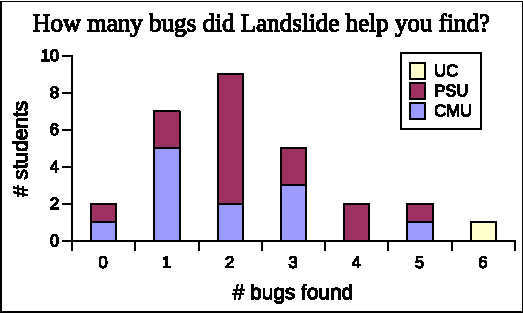
\includegraphics[width=0.42\textwidth]{survey1.pdf} &
			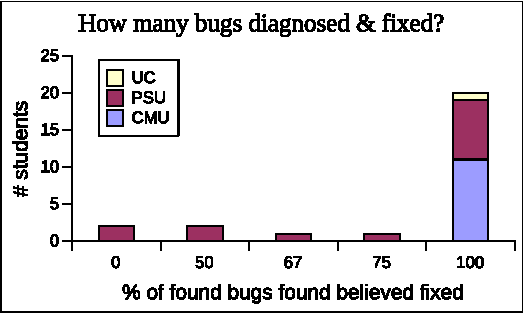
\includegraphics[width=0.42\textwidth]{survey2.pdf} \\
			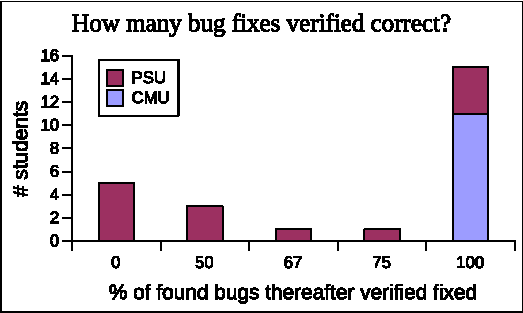
\includegraphics[width=0.42\textwidth]{survey3.pdf} &
			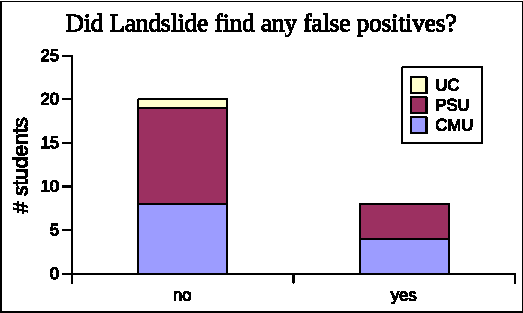
\includegraphics[width=0.42\textwidth]{survey4.pdf} \\
			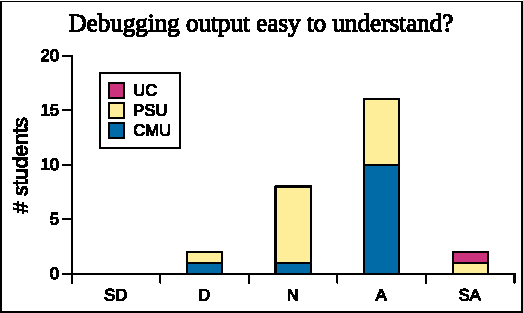
\includegraphics[width=0.42\textwidth]{survey5.pdf} &
			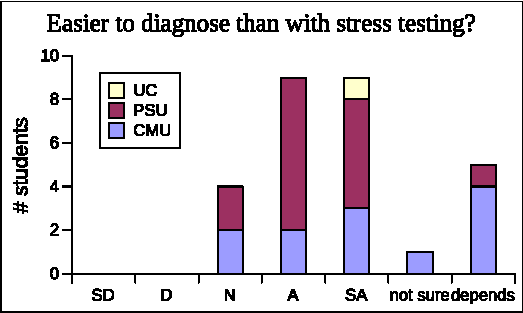
\includegraphics[width=0.42\textwidth]{survey6.pdf} \\
			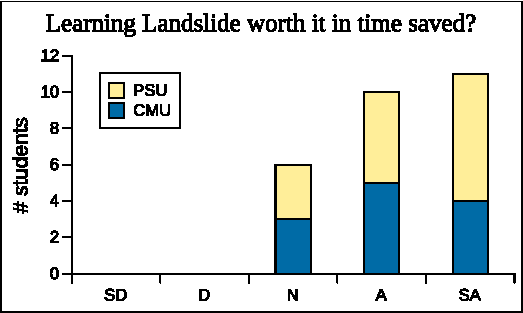
\includegraphics[width=0.42\textwidth]{survey7.pdf} &
			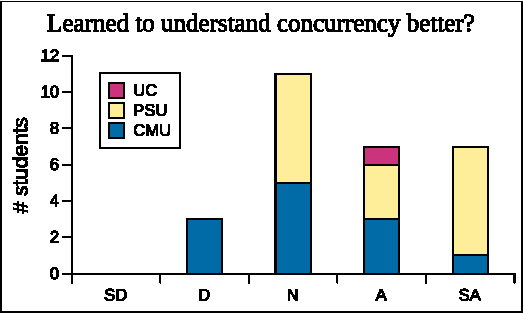
\includegraphics[width=0.42\textwidth]{survey8.pdf} \\
			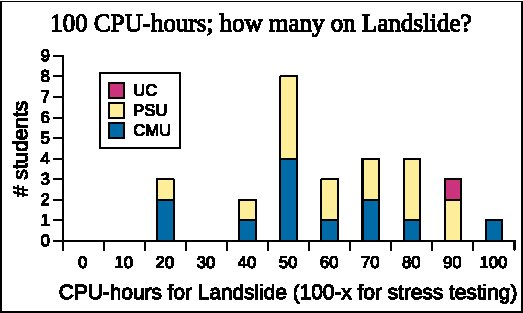
\includegraphics[width=0.42\textwidth]{survey9.pdf} &
			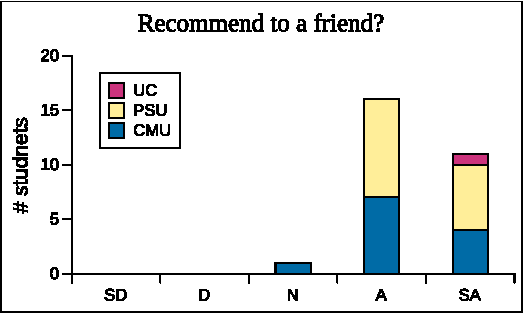
\includegraphics[width=0.42\textwidth]{survey10.pdf} \\
		\end{tabular}
	\end{center}
	\caption{Student survey responses.
	SD/D/N/A/SA stands for
	strongly disagree/\allowbreak{}disagree/\allowbreak{}neutral/\allowbreak{}agree/\allowbreak{}strongly agree.}
	\label{fig:survey}
\end{figure}

\subsubsection{Response data}

The response distributions for each of the surveys' multiple choice questions
are shown in Figure~\ref{fig:survey}.
In total, 28 students (or pairs thereof) answered the survey:
12 pairs from CMU, 15 individuals from PSU, and 1 pair from U. Chicago.
The first four questions/graphs focus on concrete debugging results,
and the latter six on the students' subjective opinions.
%
Note that two of the questions
(3 and 7 from \sect{\ref{sec:education-survey-pebbles}})
were not asked on U. Chicago's version of the survey,
so their corresponding graphs show only CMU and PSU response data.
Likewise, U. Chicago's questions 4, 8, and 10
(see \sect{\ref{sec:education-survey-pintos}}),
which were not asked on CMU's and PSU's surveys,
having only one respondent,
are not pictured;
the answers thereto were ``15-20 minutes'', ``Agree'', and ``Agree'', respectively.

The survey responses were very positive:
% TODO: corroborate this with snapshot data?
students reported being able both to diagnose and to verify as fixed the vast majority of Landslide's reported bugs,
compared Landslide favorably to stress testing,
and found the experience worthwhile and worth recommending.
Three questions with open-form answers bear further discussion:
what kind of false positives Landslide reported, % oopsative mood
reasons they found it worth recommending to a friend,
and suggestions for improving the interface
(PSU only\footnote{I thought to ask this question too late for CMU's surveys.}). % ososugichatte

\subsubsection{False positives}

Even though 71\% of students reported receiving no false positive bug reports,
the nature of Landslide's bug-detection algorithms is such
that it should ideally never report any correct behaviour as wrong,
so I consider those 29\% that did report such the most negative result among the survey responses.
They described their false positives, and I either make excuses or own up, as appropriate, as follows.
Reports from CMU students (Simics version):
\begin{enumerate}
	\item Landslide complained of a nonexistent {\tt MAGIC\_BREAK} (Simics debugging function),
		despite the student's code never invoking it.
		This arose because of technical confusion between the test program's and the shell's address spaces,
		and was subsequently fixed in commit 3f24d67 (Simics repository only).
	\item Landslide reported ``some weird errors'' and/or mysteriously crashed
		when multiple instances were run from the same directory.
		(Multiple students suffering this failure mode contacted me for support,
		though only one reported it on the survey;
		in some cases, I recall said weird errors manifesting as false positive invalid heap access reports.)
		Simultaneous Landslides can clobber certain auto-generated header and/or temporary files,
		leading to undefined behaviour.
		I introduced a guard against this in commit 977e8fb (Simics repository) and e49b5df (Bochs repository).
	\item One student reported ``Data races which I believe they are not''.
		Looking at their usage snapshots to corroborate this,
		these appear to be true, yet benign, data races
		(in several cases corresponding to {\tt mutex\_test}'s verification of the mutex's internal memory accesses
		(see \sect{\ref{sec:education-pebbles-tests}}));
		i.e., expected behaviour rather than false positive bug reports.
		Student confusion about these could be alleviated
		by improving Landslide's user interface messages when printing data race information. % uuuuuuu its already so
	\item One student complained of a bug report that, while truly a bug, showed wrong filenames and line numbers in stack traces,
		and (quite naturally) suggested that accurate stack traces would make debugging easier.
		Checking against their usage snapshots,
		this seems to be an issue with Simics's symtable's handling of assembly functions.
		The Bochs version handles these correctly.
\suspend{enumerate}
Reports from PSU students (Bochs version):
\resume{enumerate}
	\item Landslide kept crashing for one student while running {\tt paraguay}.
		This is likely due to exceeding Linux's process limit and/or exhausting the class's official VM's memory,
		which can arise when many data race candidates cause Quicksand to spawn many Landslide jobs,
		and (as on {\tt paraguay}) each with very large state spaces that must defer.
		I had been working on mitigating this problem just before beginning the PSU study;
		properly addressing it would involve improving Quicksand's memory-exhaustion detection code
		and/or making Quicksand at all aware of the process limit to begin with.
		(Note that this is not strictly a false positive bug report, just a Landslide crash.)
	\item Students who initialized child threads with a base pointer value of {\tt 0xffffffff} observed Landslide crashes,
		as it attempted to stack trace through that address and access memory that wrapped around the address space.
		(Several students contacted me about this via email, and I issued a prompt fix;
		one student later reported it on the survey.)
		Commits 0573e34 (Bochs repository) and 654f459 (Simics repository) fixed this bug.
		(Like the above, not actually a false positive bug report.)
	\item Landslide issued false invalid heap access reports to one student
		who had been using {\tt new\_pages} to allocate thread stacks ``very close'' to the {\tt malloc} heap.
		They reported this during the study and I fixed it promptly for them in commit 4a26da7 (Bochs repository only),
		then reminded me of it again in the survey.
	\item Finally, one student reported simply, ``Race condition''.
		Without the same usage snapshots to consult as I'd have for a CMU student,
		or more self-reported detail, I regrettably can offer no comment.
\end{enumerate}

\noindent
Overall, most of the issues reported as answers to the ``false positive'' survey question
were merely Landslide crashes or user interface confusion.
Those few truly erroneous bug reports (items 1, 2, and 7),
while certainly guilty of burdening % oopsative mood
students with worry over whether the problem is their own code or in Landslide itself,
are at least not too discouraging for two reasons.
Firstly, in all cases the students were able to recognize the false positive quickly enough to ask for help,
and I was able to deploy a fix and let them proceed before the project came due.
Secondly, each such problem, now having been fixed, will befall no future student again --
not to assert Landslide is completely bug-free now,
but it at least grows more and more stable with each passing semester.

\subsubsection{Reasons worthwhile}

After the question asking ``Would you recommend a friend taking OS next semester to use Landslide?'',
I asked the students for open-form reasons why or why not.
As the former question's answers were exclusively positive (only 1 student even answering ``no opinion''),
this question's answers turned out to be mostly praise.
3 students declined to answer this question;
I reproduce the rest, paraphrasing for clarity and brevity,%
\footnote{Note that most students used the term ``race condition'' rather than ``concurrency bug'',
as taught in CMU and PSU lecture material;
I replaced these while paraphrasing in accordance with \sect{\ref{sec:glossary}}.}
here.
Answers from CMU:

\begin{enumerate}
	\item Easy to use and found nontrivial bugs.
	\item Useful to find some bugs, but other types of bugs (such as memory corruption) were impossible to find with Landslide.
	\item Helped verify our atomic primitives were correct.
	\item Would recommend, but takes too much time (unclear, but seems to be referring to execution time rather than setup/usage).
	\item Tests are automated and can be left running for a long time.
		However, faced uptime issues with CMU's linux servers (which reboot every night);
		wished for a more reliable execution environment.
	\item It's pretty helpful. % lol
	\item Seems more reliable than stress tests.
	\item Found a bug not found by stress tests.
	\item Finds concurrency bugs with little effort that may be undiscovered otherwise.
		(Also provided some interface feedback here, since I didn't ask CMU students a separate question for such;
		see next section.)
	\item Easy to learn and a simple way to test our P2.
\suspend{enumerate}
Answers from PSU:
\resume{enumerate}
	\item Although didn't find any concurrency bugs for me, gives me more confidence about my code.
	\item Helpful, just didn't have a lot of time to use it.
	\item Does not make concurrency debugging easy, but definitely makes it easier.
	\item Helpful to find bugs you weren't previously aware of.
		Makes more sense to use an expressly designed tool rather than (unit/stress) tests.
	\item Helpful and easy to use.
	\item Saves time overall, can run long tests overnight.
	\item Helps to find concurrency bugs and their root causes better than stress tests.
	\item It finds the concurrency bugs you need to fix for full credit.
	\item Helpful for finding some uncommon bugs I hadn't found or wasn't looking for.
	\item Found bugs I kept overlooking, which may have taken many hours to find otherwise.
	\item Helpful for the difficult step from code being ``finished'' (scare-quotes theirs; presumably meaning ``feature-complete'')
		to getting rid of all concurrency bugs.
	\item Easy to use, setup taking no more than 5-10 minutes, and allowing being run overnight.
	\item Very efficient at concurrency testing.
		Stress test crash reports do not necessarily point to the root cause, due to memory corruption for example;
		plus bugs may not show up every time due to nondeterminism.
	\item Helped find a bug I wouldn't have found otherwise.
		Did not show an interleaving directly (i.e., did not issue a bug report),
		but reported a data race that turned out to be a concurrency bug upon inspection.
\suspend{enumerate}
Answer from U. Chicago:
\resume{enumerate}
	\item Found several subtle, legitimate bugs we wouldn't have easily caught otherwise, but made sense once revealed.
		Fixing them took little time but allowed us to proceed confidently on the next project.
		Often wished for Landslide to have been available to use during the next project as well.
\end{enumerate}

\noindent
Overall, students most commonly praised Landslide's ease of use,
its ability to find bugs that elude stress testing,
and the confidence instilled from verifying bugs had been fixed.

\subsubsection{Interface suggestions}

Lastly, I asked the PSU students for any feedback they might have on making Landslide's interface easier to use or understand.

\begin{enumerate}
	\item Requested for preemption traces to be more clear about the meaning of each stack trace in each table cell,
		and complained of inaccurate line numbers
		(likely referring to how the current behaviour indicates the line of code {\em after} a function call,
		corresponding to the {\tt call} instruction's pushed return address,
		rather than the function call itself). (This answer from CMU; see above.)
	\item Including a manual or tutorial would be helpful (presumably beyond the user guide's instructions, such as recapping the procedure shown in the lecture demo which wasn't written down anywhere).
	\item Don't print warnings about line length exceeding 80 characters (inconsistency between 15-410 and \psuos compilation options).
	\item ``It takes too long. But I guess that's impossible to fix.'' (Well, it's an open research problem to fix!)
	\item Preemption traces should explicitly indicate where in the interleaving the bug occurred.
		(Root cause identification is its own research area, but more detail is certainly possible.)
	\item Improve explanation of data races (in the user guide, perhaps).
	\item Happy with it as-is (3 students)
	\item No response (7 students)
\end{enumerate}

Though I did not ask this question on the CMU survey,
my experience handling student questions suggests CMU students
also mostly wish for
better explanations of data races and
more detail and clarity in the preemption traces.
Though I present the formal definition of data races in the lecture
(\sect{\ref{sec:education-pebbles-recruiting}})
and refer back to it in Landslide's documentation and output,
showing a concrete example
in future iterations of the user guide
would go a long way to illustrate the abstract concepts.
The preemption traces could be improved by making it clearer that the stack trace in each cell of the table
represents executing the thread in question from wherever it previously left off (or its inception)
all the way until it reaches that stack trace, then preempting it to run another thread.
They could also easily report more diagnostic information;
for example, showing the sets of memory conflicts between each thread,
annotating the type of each preemption point (yield, mutex, or data race),
and/or indicating the adversarial memory access for each data race preemption point.

\subsection{Other universities}

% TODO

%%%%%%%%%%%%%%%%%%%%%%%%%%%%%%%%%%%%%%%%%%%%%%%%%%%%%%%%%%%%%%%%%%%%%%%%%%%%%%%%

\section{Discussion}

% TODO intro text

\subsection{Bias}

% TODO: addressing bias
% well, we did the best we could(?)
% survey email: "please answer honestly rather than flatteringly" vs. studence trying to be polite
% selection bias, students who liked landslide more more likely to answer the survey at all
% TODO - u can verify the bug just by taking survey graph #1 and comparing to landslide snapshots (sep. by groups who answered survey)
% anything else?

%%%% pintos %%%% (?? this is psu not pintos)
% survey questions i WISH i had asked
% - did you have any technical difficulties w landslide that i had to intervene on
% mb anything else from timmys 2nd latest email

\subsection{Retrospect}

Human subjects research is inherently messy.
More than just trying to draw firm conclusions from
the opinions of students who are just learning concurrency to begin with,
student feedback in turn guided the constant development
of Landslide, and the experimental design itself,
as the semesters went by.
In this section I will fantasize about how I might have run more perfect experiments
granted the impossible wish of knowing then what I know now.

\subsubsection{Pebbles}

% TODO

\subsubsection{Pintos}

While part of the point of this experimental design was to evaluate Landslide as a grading tool in the hands of TAs,
I would be remiss to mention that I also feared the automatic annotation process would not be as robust as the P2 version.
Indeed, while helping Kevin get oriented with using Landslide,
I implemented
several
fixes/improvements to the setup scripts
as we found student kernels that failed to automatically annotate
(for example, those with {\tt ready\_list} changed to an array,
as described in \sect{\ref{sec:education-pintos-instrumentation}}).
Had we given Landslide directly to students that semester,
the students themselves would have had to email me for tech support.

I attribute the low participation rate of Pintos students to P2 students to two major factors:
one, not incentivizing the students to directly improve their grades
(instead offering only the vague promise of a ``learning experience'' debugging their code only after handin),
and two, not traveling to the university to introduce the research topic in an in-person lecture
(leaving the students potentially confused about what advantage, if any, was offered over stress testing).
Hypothetically, I could have achieved greater user study participation
either by offering extra credit to students
or by offering an autograder-like interface for students to receive bug reports before their deadlines instead of after
(either way requiring a more rigorous IRB review process).

\subsection{Future educational use}

% TODO: para for pebbles; discuss with dave

Regarding non-research use in Pintos classes,
Landslide can now handle a considerably wider variety of student implementation quirks
on account of the fixes from this time (\sect{\ref{sec:education-pintos-instrumentation}}).
In its current shape I would recommend it for TA use grading,
but not necessarily directly to students without someone familiar with the codebase on immediate hand for tech support.
However, I also believe Landslide's success in these user studies,
provided me present to handle technical issues,
serves as testament for stateless model checking in general in the educational theatre.
While Pintos's kernel-level environment presents a unique challenge for concurrency testing,
other, more readily automatic model checkers for user-space programs,
such as dBug \cite{dbug-ssv},
could easily be used on other thread-library-like programming projects at any university.

